\documentclass{article}
\usepackage{enumerate}
\usepackage{amsmath}
\usepackage{amssymb}
\usepackage{graphicx}
\usepackage{subfigure}
\usepackage{geometry}
\usepackage{color}
\usepackage{bm}
\usepackage{indentfirst}

\begin{document}

\vspace*{0.25cm}

\hrulefill

\thispagestyle{empty}

\begin{center}
\begin{large}
\sc{UM--SJTU Joint Institute \vspace{0.3em} \\ Physics Laboratory \\(Vp141)}
\end{large}

\hrulefill

\vspace*{5cm}
\begin{Large}
\sc{{Laboratory Report}}
\end{Large}

\vspace{2em}

\begin{large}
\sc{{Exercise 3
\vspace{0.5em}

Simple Harmonic Motion:\\
Oscillations in Mechanical Systems
}}
\end{large}
\end{center}


\vfill

\begin{table}[h!]
\flushleft
\begin{tabular}{lll}
Name: Yihao Liu \hspace*{2em}&
ID: 515370910207\hspace*{2em}\\
Name: Guangzheng Wu \hspace*{2em}&
ID: 515370910014\hspace*{2em}
& Group: 7\\


\\

Date: 8 June 2016 

\end{tabular}
\end{table}

\hfill
\begin{tiny}
[rev. 1.0]
\end{tiny}
\newpage

\section{Introduction}

The main objective of this exercise is to study simple harmonic oscillation. You will
learn how to find the spring constant and effective mass of a spring, and how to use the
air track. We will analyze the relationship between the oscillation period and the mass
of the oscillator, check whether the oscillation period depends on the the amplitude, and
examine the relationship between the maximum speed and the amplitude.
\\

There are various kinds of periodic motion in nature, among which the simplest and
the most fundamental one is the simple harmonic motion, where the restoring force is
proportional to the displacement from the equilibrium position and as a result, the position
of a particle depends on time as the sine (or cosine) function. Discussion of the simple
harmonic motion is a basis for studying more complex situations.

\subsection{Hooke’s Law}

Within the elastic limit of deformation, the force F x needed to be applied in order to
stretch or compress a spring by the distance x is proportional to that distance, i.e.,

\begin{equation}\label{eq-1}
F_x=kx
\end{equation}

where $k$ is a constant (called the spring constant) characterizing how easy it is to deform
the spring. This constant will be found in the present exercise using a measurement device
called the Jolly balance. The linear relation (\ref{eq-1}), between the force and the deformation, is
known as the Hooke’s Law. According to Newton’s third law of dynamics, the spring exerts
a reaction force (called the elastic force) of the same magnitude but opposite direction. As
this force tries to restore the system back to the equilibrium, it is known as the restoring
force.

\subsection{Equation of Motion of the Simple Harmonic Oscillator}

As shown in Figure \ref{fig-1}, an object with mass $M$ is set on an air track with a spring
attached to both of its sides. The purpose of using the air track is to eliminate frictional
forces between moving surfaces. The other ends of the springs are fixed to the air track.
The spring constants $k_1$ and $k_2$ are to be measured with the Jolly balance. The origin
($x$ = 0) of the coordinate system is set at the equilibrium position of the mass $M$ .
Assuming that the masses of the springs can be ignored, and neglecting damping in the
system, the elastic (restoring) forces of the springs are the only forces acting on mass $M$ .
According to Newton’s second law of dynamics, the equation of motion of mass $M$ is

\begin{figure}[!h]
	\centering
	\includegraphics[width=10cm]{fig-1.png}
	\caption{Mass-spring system.
	\label{fig-1}}
\end{figure}

\begin{equation}\label{eq-2}
M\frac{d^x}{dt^2}+(k_1+k_2)x=0
\end{equation}

The general solution to Eq. (\ref{eq-2}) is

\begin{equation}\label{eq-3}
x(t)=A\cos(\omega_0t+\varphi_0)
\end{equation}

where $\omega_0=\sqrt{(k_1+k_2)/M}$ is the natural angular frequency of the oscillations, $A$ is their
amplitude, and $\varphi_0$ is the initial phase. The natural angular frequency is determined by
the parameters of the system itself, whereas the initial phase is determined by initial
conditions. The natural period of oscillation is

\begin{equation}\label{eq-4}
T=\frac{2\pi}{\omega}=2\pi\sqrt{\frac{M}{k_1+k_2}}
\end{equation}

In this exercise, the relationship between the oscillation period and the mass of the oscillator will be studied.

\subsection{Effect of the Mass of the Spring}

Whenever the mass of the springs cannot be ignored, we take it into account in terms
of the so-called effective mass. The effective mass of the oscillator is the sum of the mass
of the object and the effective mass of the spring. When we take the effective mass of the
spring into account, the angular frequency of the system can be expressed as

\begin{equation}\label{eq-5}
\omega_0=\frac{k_1+k_2}{M+m+0}
\end{equation}

where $m_0$ is the effective mass of the spring, which is 1/3 of the actual mass of the spring.

\subsection{Mechanical Energy in Harmonic Motion}

The elastic potential energy for a spring-mass system is $U=kx^2/2$ and the kinetic
energy of an oscillating mass $m$ is $K=mv^2/2$.\\

At the equilibrium position ($x=0$), the speed of the mass is maximum $v=v_{max}$ .
At this point the total mechanical energy is equal to maximum kinetic energy $K_{max}$ . On
the other hand, at maximum displacement ($x=\pm A$) the mass is instantaneously at rest,
i.e. $v=0$, and the contribution to the total mechanical energy is due to the potential
energy only, which is at its maximum $U_{max}$ . In the absence of non-conservative forces
(such as frictional forces or drag forces), the total mechanical energy is conserved and
$K_{max}$ = $U_{max}$ , which implies

\begin{equation}\label{eq-5}
k=\frac{mv_{max}^2}{A^2}
\end{equation}

\section{Experimental setup}

The measurement equipment consists of the following elements: springs, Jolly balance,
air track, electronic timer, electronic balance, and masses.\\

\begin{figure}[!t]
	\centering
	\includegraphics[width=10cm]{fig-2.png}
	\caption{Jolly balance.
	\label{fig-2}}
\end{figure}

In order to measure the spring constant using the Jolly balance, we need to place the
small mirror $C$ (see Figure \ref{fig-2}) in the tube $D$ and make three lines coincide: the line on
on the mirror, the line on the glass tube and its reflection in the mirror. First, without
adding any weight on the bottom end of the spring, tune the knob $G$ and make the three
lines coincide. Then read the scale $L_1$ .\\

Second, add mass $m$ to the bottom of the spring. The spring is stretched and the
three lines no longer coincide. Tune knob $G$ to make them into one line again and read
the corresponding number on scale $L_2$ . The spring constant may be then found as

\begin{equation}\label{eq-6}
k=\frac{mg}{L_2-L_1}
\end{equation}

When you have a series of measurements, for different masses $m$, you may use the least
square method to estimate the spring constant by finding a linear fit to the data.\\

\begin{figure}[!t]
	\centering
	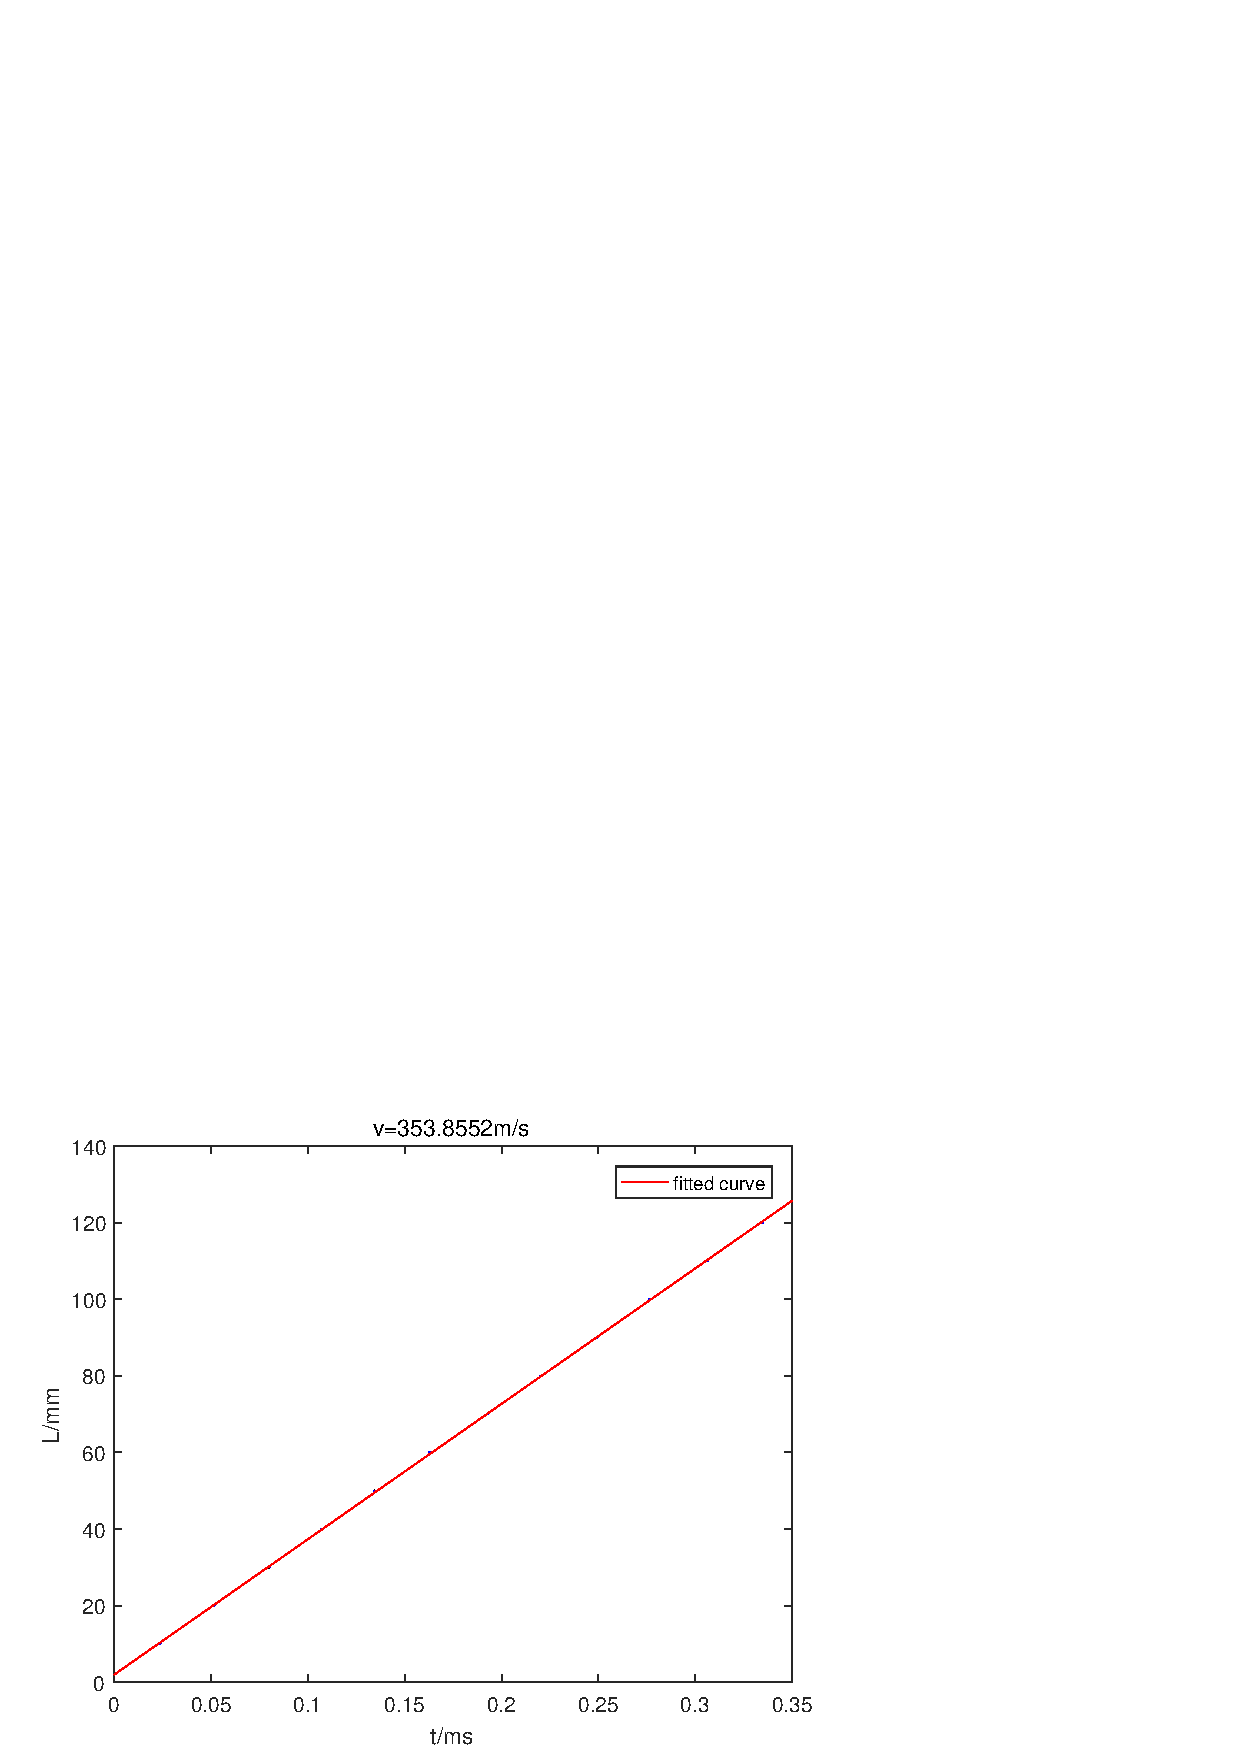
\includegraphics[width=10cm]{fig-3.png}
	\caption{The experimental setup.
	\label{fig-3}}
\end{figure}

\begin{figure}[!t]
	\centering
	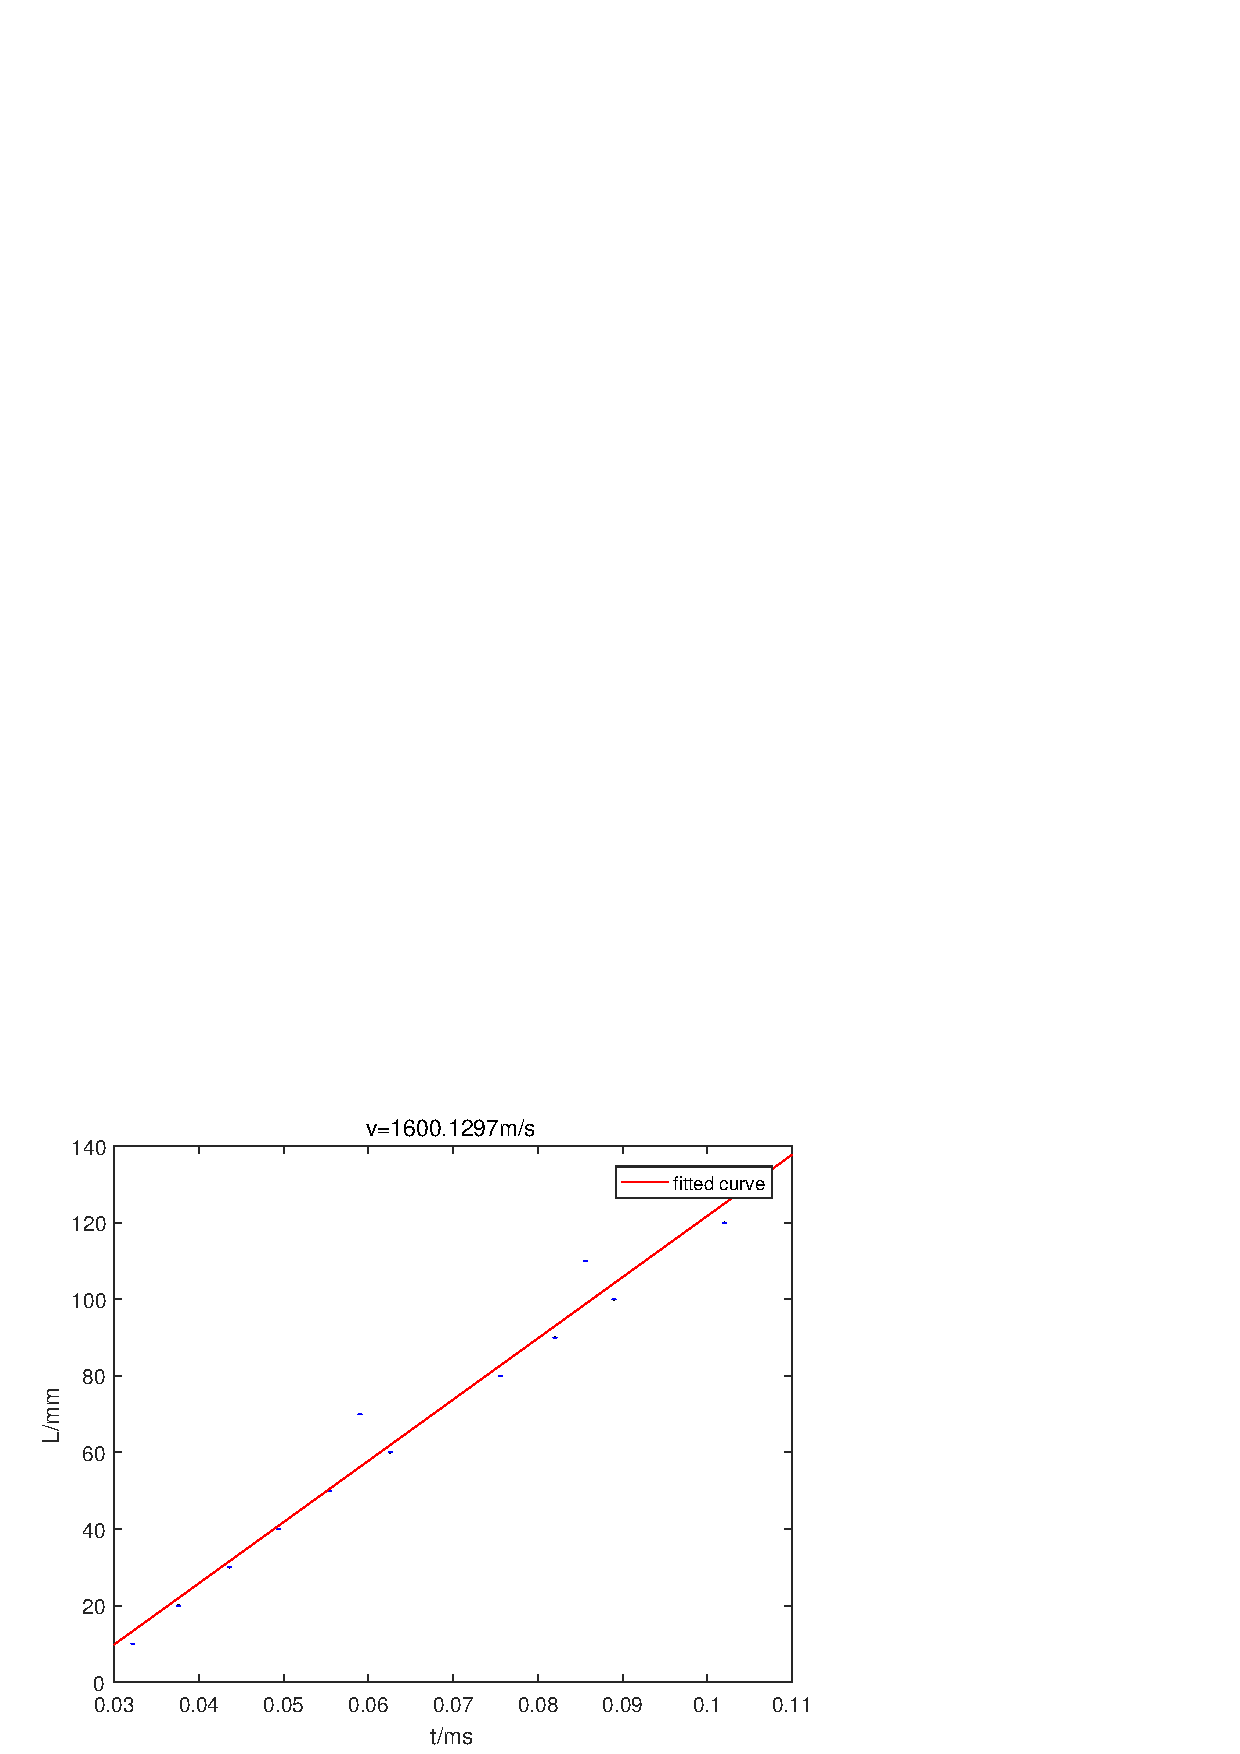
\includegraphics[width=7cm]{fig-4.png}
	\caption{The U-shape shutter.
	\label{fig-4}}
\end{figure}

A photoelectric measuring system consists of two photoelectric gates and an electronic
timer. When a shutter placed on the object passes a gate, it blocks the light emitted from
the light source at the top of the gate, and the receiver sends a signal to the electronic
timer. Please note that for period measurements we use, we use the I-shape shutter.\\

When measuring the speed of the object, we use a U-shaped shutter (Figure \ref{fig-4}), so
that the light is blocked twice during a pass. The timer will then record the time interval
$\Delta t$ between the two generated signals. After the distance $\Delta x=\frac{1}{2}(x_{in}+x_{out})$ between
the two arms of the U-shape shutter is measured, the speed of the object at the point of
passing the gate is calculated as $v=\Delta x/\Delta t$.

\section{Measurement}

\subsection{Spring Constant}

\begin{enumerate}
\item
Adjust the Jolly balance to be vertical: Attach the spring and the mirror as shown
in Figure \ref{fig-2}. Add a 20 g preload and adjust knob $I_1$ and $I_2$ to make sure the mirror
can move freely through the tube.\\
\\
Check whether the Jolly balance is parallel to the spring, and adjust knobs if necessary. You should look at the balance from two orthogonal directions: from one
direction, adjust the balance to be parallel to the spring; from the direction orthogonal to the previous one, check if the balance coincides with the spring.
\item
Adjust knob $G$ and make the three lines in the tube coincide. Adjust the position
of the tube to set the initial position $L_0$ within 5.0 ∼ 10.0 cm.
\item
Record the reading $L_0$ on the scale, add mass $m_1$ and record $L_1$ .
\item
Keep adding masses and take measurements for six different positions. The order
of the masses should be recorded.
\item
Estimate the spring constant $k_1$ using the least square method.
\item
Replace spring 1 with spring 2, repeat the measurements and calculate $k_2$ .
\item
Remove the preload and repeat the measurement for springs 1 and 2 connected in
series. Calculate $k_3$ and compare it with the theoretical value.
\end{enumerate}

\subsection{Relation between the Oscillation Period $T$ and the Mass of the Oscillator $M$}

\begin{enumerate}[(a)]
\item
Adjust the air track so that it is horizontal.\\
\\
Caution: Do not place anything on the air track before you turn on the air pump.
	\begin{enumerate}[1.]
	\item
	Turn on the air pump and check if any of the holes on the air track are blocked.
Call the instructor for help if you find blocked holes.
	\item
	Place the object (cart) on the track without any initial velocity. Adjust the track
until the object moves slowly back and forth in both directions.\\
	Adjustment method. The air track has three knobs at the bottom: two on one side
and another one on the other side. You can only adjust that single knob.
	\end{enumerate}
	
\item
Horizontal air track
	\begin{enumerate}[1.]
	\item
	Attach springs to the sides of the cart, and set up the I-shape shutter. Make sure
that the photoelectric gate is at the equilibrium position.
	\item
	Add weight $m_1$ . Let the cart oscillate about the photoelectric gate. The amplitude
of oscillations should be about 5 cm. Release the cart with a caliper or a ruler. Set
the timer into the ``T'' mode. The timer in this mode will automatically record
the time of 10 oscillation periods. Record the mass of the cart and the period.
	\item
	Add weights to the object, repeat Step 2 and take measurements for 5 times.
	\item
	Analyze the relation between $M$ and $T$ by plotting a graph.
	\end{enumerate}
	
\item
Inclined air track
	\begin{enumerate}[1.]
	\item
	Inclination of the air track is controlled with plastic plates. Place them under the
air track, using three plates at a time.
	\item
	Repeat the steps in (b) for two different inclinations (i.e., with 3 and 6 plates beneath the air track).
	\item
	Discuss the relation between $M$ and $T$ by plotting a graph.
	\end{enumerate}
		
\end{enumerate}

\subsection{Relation Between the Oscillation Period $T$ and the Amplitude $A$}

\begin{enumerate}
	\item
	Keep the mass of the cart unchanged and change the amplitude (choose 6 different
values). The recommended amplitude is about 5.0/ 10.0/ 15.0/ ... /30.0 cm.
	\item
	Apply linear fit to the data and comment on the relation between the oscillation period
$T$ and the amplitude $A$ based on the correlation coefficient $\gamma$.
\end{enumerate}

\subsection{Relation Between Maximum Speed and the Amplitude}

\begin{enumerate}
	\item
	Measure the outer distance x out and the inner distance $x$ in of the U-shape shutter by
a caliper. Calculate the distance $\Delta x=(x_{out}+x_{in})/2$.
	\item
	Change the shutter from I- to U-shape. Set the timer into the ``$S_1$'' mode. Let the cart
oscillate. Record the second readings of the time interval $\Delta t$ only if the two subsequent
readings show the same digits to the left of the decimal point.
	\item
	Change the amplitude (choose 6 different values). The recommended amplitude is
about 5.0/ 10.0/ 15.0/ ... /30.0 cm.
	\item
	Measure the maximum speed $v_{max}$ for different values of the amplitude $A$. Obtain the
spring constant from Eq. (\ref{eq-6}). Compare this result to that of the first part.
\end{enumerate}



\subsection{Mass measurement}
\begin{enumerate}
	\item
	Adjust the electronic balance every time before you use it. The level bubble should be
in the center of the circle.
	\item
	Add weights according to a fixed order. Weigh the cart with the I-shape shutter and
with the U-shape shutter. Measure the mass of spring 1 and spring 2.
	\item
	Record the data only after the circular symbol on the scales display disappears.
\end{enumerate}

\newpage

\section{Results}

\subsection{Spring Constant}

The measurement of length $L$ was shown in Table \ref{tab-1}.\\

\begin{table}[!h]
\begin{center}
\begin{tabular}{|c|c|c|c|}
\hline
\textit{Measurement} & spring 1 [cm] $\pm$ 0.01[cm] &
spring 2 [cm] $\pm$ 0.01[cm] & series [cm] $\pm$ 0.01[cm]\\
\hline
$L_0$	&	6.14	&	6.08	&	20.82\\
$L_1$	&	8.27	&	8.14	&	25.06\\
$L_2$	&	10.35	&	10.23	&	29.25\\
$L_3$	&	12.34	&	12.34	&	33.28\\
$L_4$	&	14.36	&	14.45	&	37.54\\
$L_5$	&	16.49	&	16.55	&	41.61\\
$L_6$	&	18.60	&	18.73	&	45.89\\
\hline
\end{tabular}
\caption{Spring constant measurement data.}
\label{tab-1}
\end{center}
\end{table}

According to the mass data in Table \ref{tab-5}, use MATLAB to plot the spring constant $k$ with the least square method and the result was shown in Figure \ref{fig-5}.\\

The spring constant of spring 1 is fit to be $k=2.2581\pm6.1769\times10^{-4}N/m$\\

The spring constant of spring 2 is fit to be $k=2.2138\pm7.8746\times10^{-4}N/m$\\

The spring constant of the series is fit to be $k=1.12\pm5.4961\times10^{-4}N/m$\\

The theoretical value is $$k=\frac{k_1k_2}{k_1+k_2}\approx1.1178$$

It is similar to the experimental value.



\begin{figure}[h!]
	\centering
	\subfigure[$k_1$]{
	\label{Fig.sub.1}
	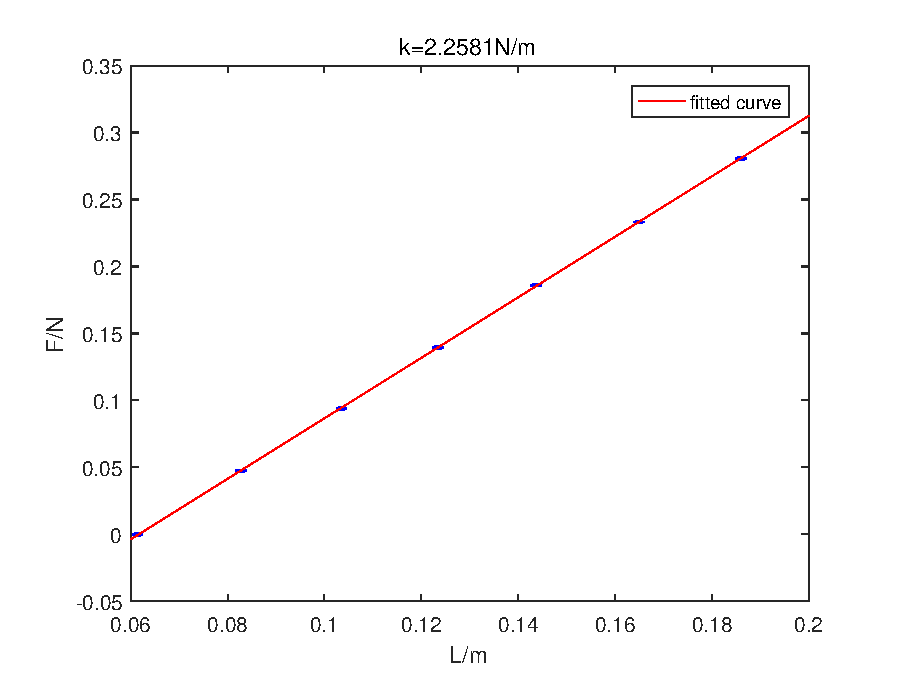
\includegraphics[width=7cm]{fit-1.eps}}
	\subfigure[$k_2$]{
	\label{Fig.sub.2}
	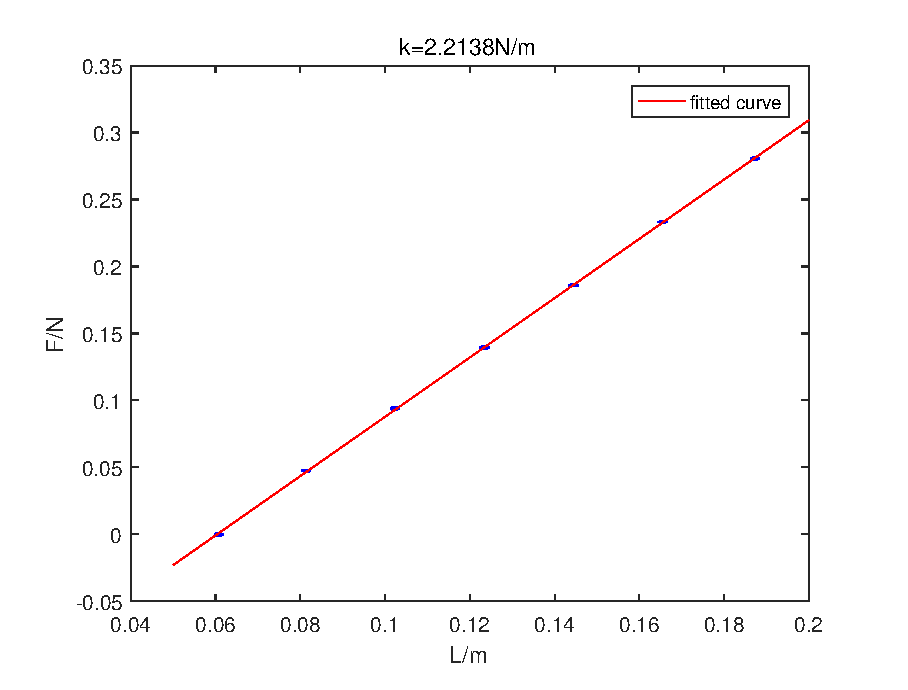
\includegraphics[width=7cm]{fit-2.eps}}
	\subfigure[series]{
	\label{Fig.sub.3}
	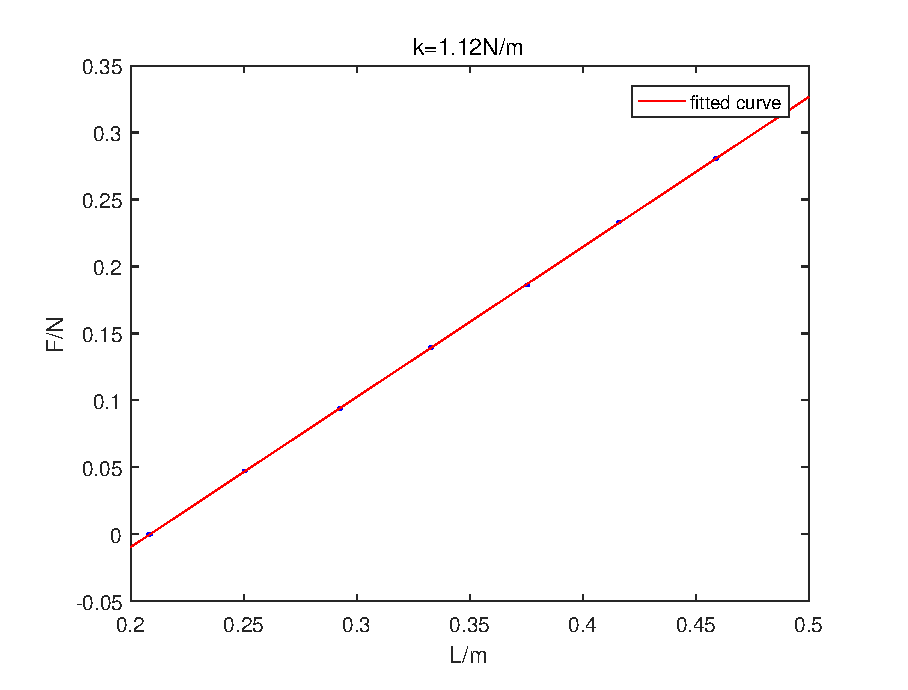
\includegraphics[width=7cm]{fit-3.eps}}
	\caption{Fit of spring constant.}
	\label{fig-5}
\end{figure}

\newpage

\subsection{Relation between the Oscillation Period $T$ and the Mass of the Oscillator $M$}

\begin{table}[!h]
\begin{center}
\begin{tabular}{|c|c|c|c|}
\hline
\multicolumn{4}{|c|}{ten period [ms] $\pm$ 0.1 [ms]}\\
\hline
\textit{Measurement} & horizontal & incline 1 & incline 2\\
\hline
$m_1$	&	12929.0	&	12925.7	&	12922.9\\
$m_2$	&	13084.7	&	13081.8	&	13077.7\\
$m_3$	&	13234.8	&	13230.4	&	13227.0\\
$m_4$	&	13388.8	&	13384.1	&	13377.8\\
$m_5$	&	13536.9	&	13532.3	&	13529.7\\
$m_6$	&	13687.0	&	13684.2	&	13679.4\\
\hline
\end{tabular}
\caption{Measurement data for the $T$ vs. $M$ relation.}
\label{tab-2}
\end{center}
\end{table}

The measurement of ten periods $10T$ was shown in Table \ref{tab-2}.\\

According to the mass data in Table \ref{tab-5}, use MATLAB to plot $T$ vs. $M$ with the least square method and the result was shown in Figure \ref{fig-6}.\\

The horizontal is fit to be $k=3.184\pm0.4141ms/g$\\

The incline 1 is fit to be $k=3.1824\pm0.3503ms/g$\\

The incline 2 is fit to be $k=3.1773\pm0.2921ms/g$\\

It can be concluded that $T$ is in proportion to $M$ and Then the incline became larger, the ratio became smaller.

\begin{figure}[h!]
	\centering
	\subfigure[horizontal]{
	\label{Fig.sub.1}
	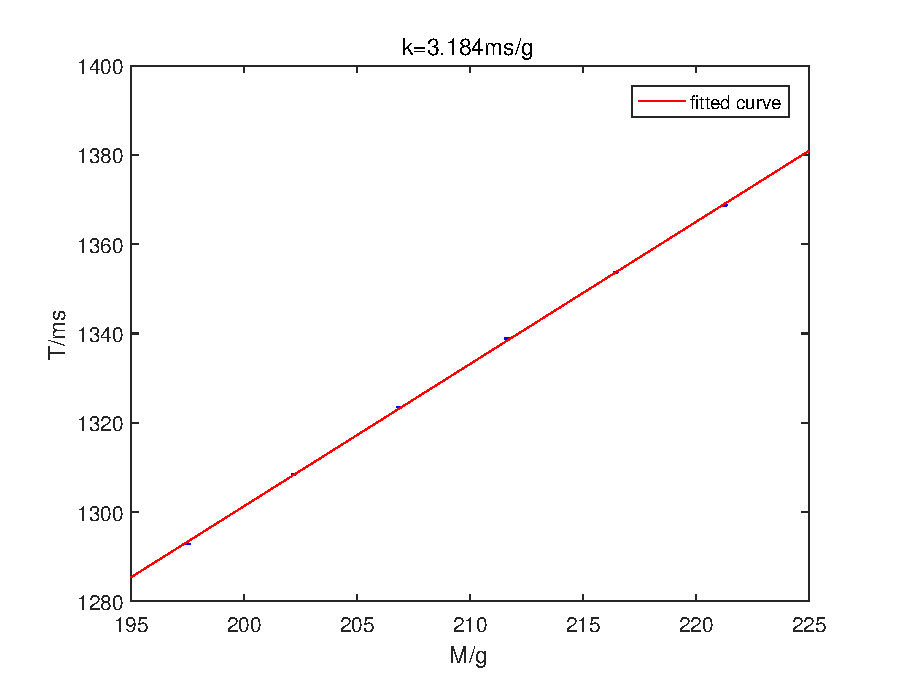
\includegraphics[width=7cm]{fit-4.eps}}
	\subfigure[incline 1]{
	\label{Fig.sub.2}
	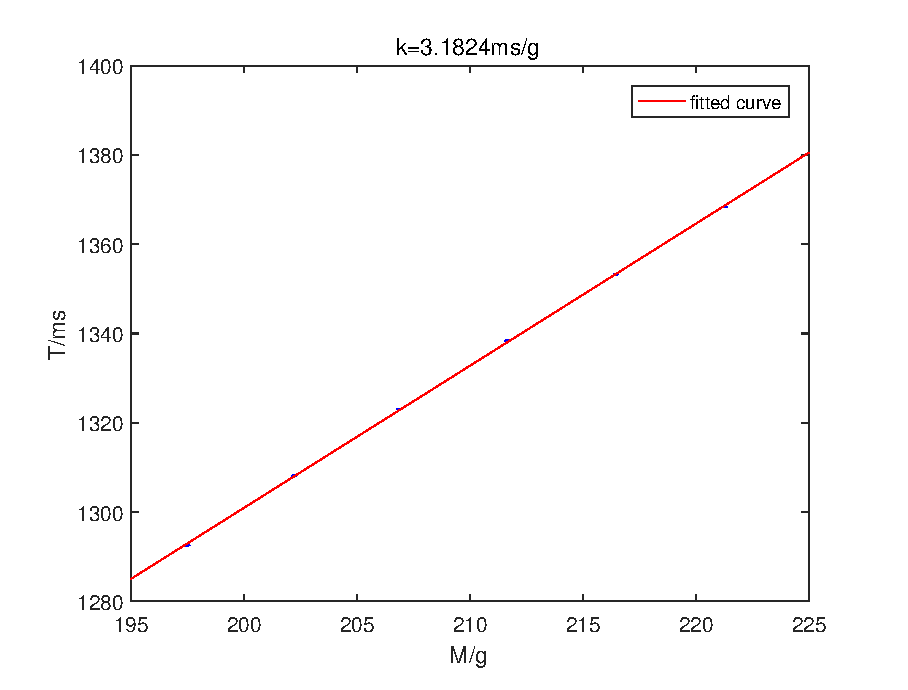
\includegraphics[width=7cm]{fit-5.eps}}
	\subfigure[incline 2]{
	\label{Fig.sub.3}
	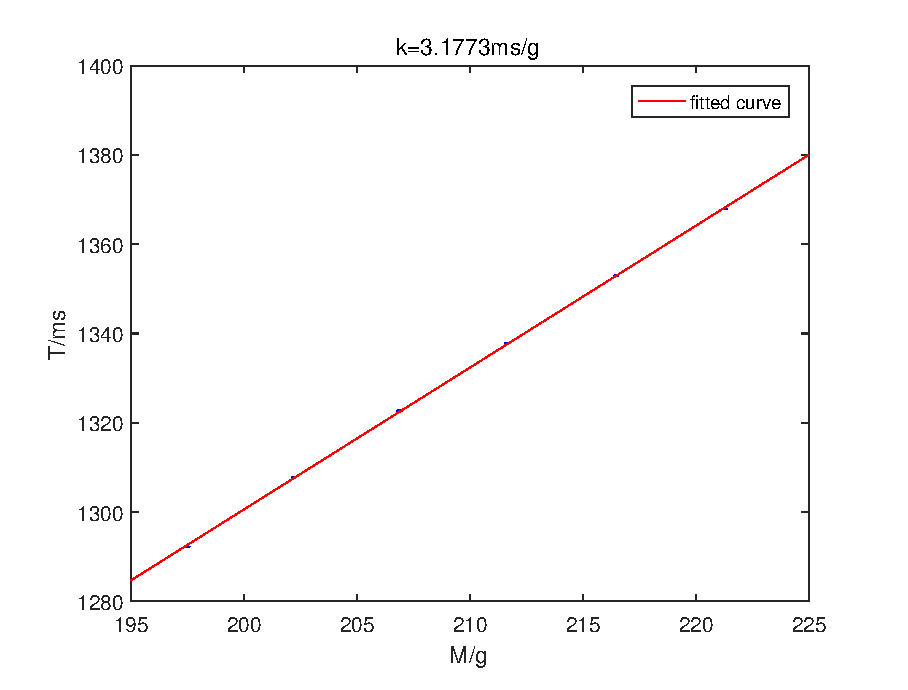
\includegraphics[width=7cm]{fit-6.eps}}
	\caption{Fit of $T$ vs. $M$.}
	\label{fig-5}
\end{figure}

\newpage

\subsection{Relation Between the Oscillation Period $T$ and the Amplitude $A$}

The measurement of ten periods $10T$ was shown in Table \ref{tab-3}.\\

\begin{table}[!h]
\begin{center}
\begin{tabular}{|c|c|c|}
\hline
\textit{Measurement} & A [cm] $\pm$ 0.1 [cm] & ten period [ms] $\pm$ 0.1 [ms]\\
\hline
1	&	5.0		&	12770.7\\
2	&	10.0	&	12759.3\\
3	&	15.0	&	12754.3\\
4	&	20.0	&	12751.0\\
5	&	25.0	&	12752.4\\
6	&	30.0	&	12782.1\\
\hline
\end{tabular}
\caption{Data for the $T$ vs. $A$ relation.}
\label{tab-3}
\end{center}
\end{table}

We can find that there is no relationship between $T$ and $A$ according to Figure \ref{fig-6}

\begin{figure}[!h]
	\centering
	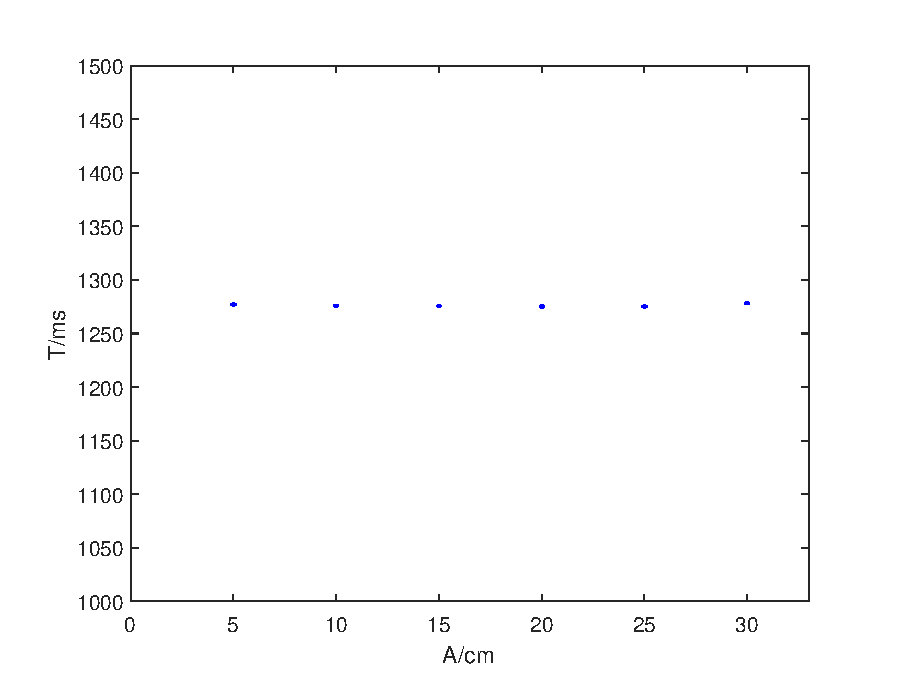
\includegraphics[width=10cm]{fig-6.eps}
	\caption{$T$ vs. $A$ relation.
	\label{fig-6}}
\end{figure}

\subsection{Relation Between Maximum Speed and the Amplitude}

The measurement of $\Delta t$ was shown in Table \ref{tab-4}.\\

\begin{table}[!h]
\begin{center}
\begin{tabular}{|c|c|c|}
\hline
\textit{Measurement} & A [cm] $\pm$ 0.1 [cm] & $\Delta t$ [ms] $\pm$ 0.01 [ms]\\
\hline
1	&	5.0		&	40.19\\
2	&	10.0	&	20.12\\
3	&	15.0	&	13.51\\
4	&	20.0	&	10.18\\
5	&	25.0	&	8.15\\
6	&	30.0	&	6.88\\
\hline
\hline
\textit{Measurement} & $x_{in}$ [cm] $\pm$ 0.002 [cm] & $x_{out}$ [cm] $\pm$ 0.002 [cm]\\
\hline
1	&	0.450	&	1.538\\
2	&	0.456	&	1.540\\
3	&	0.452	&	1.546\\
\hline
\end{tabular}
\caption{Data for the $v_{max}^2$ vs. $A$ relation.}
\label{tab-4}
\end{center}
\end{table}

We can first calculate $\Delta x$ by the formula
$$\Delta x=\frac{1}{2}(x_{out}+x_{in})=\frac{1}{6}\sum_{i=1}^3(x_{out}+x_{in})=0.997\pm0.002cm$$

Use MATLAB to plot $v_{max}^2$ vs. $A$ with the least square method and the result was shown in Figure \ref{fig-7}.\\

\begin{figure}[!h]
	\centering
	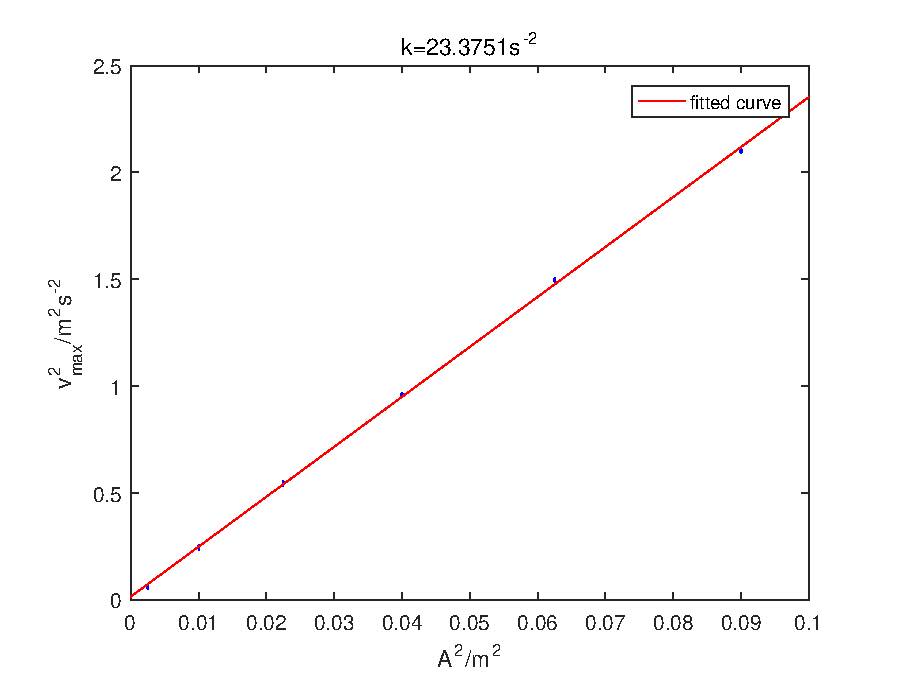
\includegraphics[width=10cm]{fig-7.eps}
	\caption{$v_{max}^2$ vs. $A$ relation.
	\label{fig-7}}
\end{figure}

where
$$k=23.3751\pm0.0160s^{-2}$$

\newpage

\subsection{Mass measurement}

The measurement of mass was shown in Table \ref{tab-5} and Table \ref{tab-6}.\\

\begin{table}[!h]
\begin{center}
\begin{tabular}{cc}
\hline
\textit{Measurement} & $m$ [g] $\pm$ 0.01 [g] \\

\hline
1	&	4.84\\
2	&	9.57\\
3	&	14.22\\
4	&	18.99\\
5	&	23.80\\
6	&	28.64\\

\hline
\end{tabular}
\caption{Weight measurement data.}
\label{tab-5}
\end{center}
\end{table}


\begin{table}[!h]
\begin{center}
\begin{tabular}{|cc|}
\hline
object with I-shape & $m_{obj}$ [g] $\pm$ 0.01[g]\\
\hline
\multicolumn{2}{|c|}{185.54}\\
\hline
object with U-shape & $m_{obj}$ [g] $\pm$ 0.01[g]\\
\hline
\multicolumn{2}{|c|}{186.14}\\
\hline
mass of spring 1 & $m_{spr1}$ [g] $\pm$ 0.01[g]\\
\hline
\multicolumn{2}{|c|}{10.63}\\
\hline
mass of spring 2 & $m_{spr2}$ [g] $\pm$ 0.01[g]\\
\hline
\multicolumn{2}{|c|}{10.74}\\
\hline
equivalent mass & $M_0=m_{obj}+\frac{1}{2}m_{spr1}+\frac{1}{2}m_{spr2}$ [g]\\
\hline
\multicolumn{2}{|c|}{192.66}\\
\multicolumn{2}{|c|}{193.26}\\
\hline

\end{tabular}
\caption{Mass measurement data.}
\label{tab-6}
\end{center}
\end{table}

\newpage

\section{Measurement uncertainty analysis}

\subsection{Uncertainty of Spring Constant}

MATLAB gives the uncertainty in the form of RMSE.

$$u_{k1}=6.1769\times10^{-4}N/m$$
$$u_{k2}=7.8746\times10^{-4}N/m$$
$$u_{series}=5.4961\times10^{-4}N/m$$

\subsection{Uncertainty of Relation between $T$ and $M$}

MATLAB gives the uncertainty in the form of RMSE.

$$u_{horizontal}=0.4141ms/g$$
$$u_{incline_1}=0.3503ms/g$$
$$u_{incline_2}=0.2921ms/g$$

\subsection{Uncertainty of Relation between $v_{max}^2$ and $A^2$}

MATLAB gives the uncertainty in the form of RMSE.

$$u_{k}=0.0160s^{-2}$$

The measurement of $\Delta x$ was type-A uncertainty, so
$$u_{\Delta x}=0.002cm$$

The uncertainty of $v_{max}^2$ is found by applying the uncertainty propagation formula

$$u_{v_{max}^2}=\sqrt{\left(\frac{\partial v_{max}^2}{\partial\Delta x}\right)^2u_{\Delta x}^2+\left(\frac{\partial v_{max}^2}{\partial\Delta t}\right)^2u_{\Delta t}^2}
=\sqrt{\frac{4\Delta x^2u_{\Delta x}^2}{\Delta t^4}+\frac{4\Delta  x^4u_{\Delta t}^2}{\Delta t^6}}$$

\begin{align*}
u_1=0.0004    \\
u_2=0.0026    \\
u_3=0.0084    \\
u_4=0.0192    \\
u_5=0.0372    \\
u_6=0.0616
\end{align*}

\newpage

\section{Conclusion}

We study simple harmonic oscillation in this experiment.\\

We learned how to find the spring constant and effective mass of a spring, and how to use the
air track. We also analyzed the relationship between the oscillation period and the mass
of the oscillator, check whether the oscillation period depends on the the amplitude, and
examine the relationship between the maximum speed and the amplitude.\\

We can simply find the formula $F=kx$ according to the results in part (a), and when two springs are connected the result was found to be 
$$k=\frac{k_1k_2}{k_1+k_2}$$

Then we can also find that the period of the oscillator has to connection with the amplitude, but is proportion to the mass. And when the plane was inclined, the ratio would become smaller\\

The square of the maximum speed of oscillator is proportion to the amplitude because of the energy rule.\\

\section{Reference}

\begin{enumerate}[(a)]
	\item
	Qin Tian, Zheng Huan, Li Yingyu, Mateusz Krzyzosiak, VP141 Exercise 3, Simple Harmonic Motion: Oscillations in Mechanical Systems, based on materials provided by the Department of Physics, Shanghai Jiaotong University.
\end{enumerate}

\end{document}
